\documentclass[11pt]{amsart}

\usepackage{amsmath,amssymb,graphicx,bbm}
\usepackage{amsthm,verbatim}
\usepackage{mathrsfs,mathtools}

\usepackage[footnotesize,bf]{caption}
\usepackage[left=1.1in,right=1.1in,top=1in]{geometry}

\usepackage{mathdefs}

%% Patch for amsart date
\usepackage{etoolbox}
\makeatletter
\patchcmd{\@maketitle}
  {\ifx\@empty\@dedicatory}
  {\ifx\@empty\@date \else {\vskip3ex \centering\footnotesize\@date\par\vskip1ex}\fi
   \ifx\@empty\@dedicatory}
  {}{}
\patchcmd{\@adminfootnotes}
  {\ifx\@empty\@date\else \@footnotetext{\@setdate}\fi}
  {}{}{}
\makeatother
%%

\title{Project 0: Characteristics for wave problems}
\author{Anka Chen}
\date{\today}

\begin{document}
\maketitle

\section{The scalar wave equation and characteristics}
Consider the one-dimensional scalar wave equation with periodic boundary conditions,
\begin{subequations}\label{eq:wave}
  \begin{align}\label{eq:wave-pde}
    u_t + a(x) u_x &= 0, & t &> 0, & x &\in [-1,1) \\\label{eq:wave-ic}
  u(x,0) &= u_0(x), & u(-1,t) &= u(1,t).
\end{align}
\end{subequations}
Here, $a(x)$ is a given function that is assumed to be Lipschitz continuous and $u_0$ is a smooth function. We solve this problem via the method of characteristics. This method observes that, if $X(t)$ is a trajectory that is the solution to the ordinary differential equation,
\begin{align}\label{eq:X-ode}
  X'(t) &= a(X(t)), & X(0) = x_0,
\end{align}
then the function $u(X(t), t)$ obeys
\begin{align}\label{eq:char-ode}
  \ddx{t} u(X(t),t) = u_x(X(t),t) X'(t) + u_t(X(t),t) = u_x(X,t) a(X) + u_t(X,t) \stackrel{\eqref{eq:wave-pde}}{=} 0.
\end{align}
Here, we define the solution $X$ to \eqref{eq:X-ode} periodically on $[-1,1)$. Thus, the value of $u(X(t),t)$ is constant in time so that
\begin{align}\label{eq:char-result}
  u(X(t),t) = u(X(0),0) \stackrel{\eqref{eq:wave-ic}}{=} u_0(x_0).
\end{align}
Thus, given $x_0 \in [-1,1)$, we can solve \eqref{eq:char-ode} forward in time with an \textit{ordinary} differential equation solver, and obtain the value of $u(X(t),t)$, effectively solving \eqref{eq:wave}. 

  There is one technicality in this result: we cannot use the result above to evaluate $u(x,t)$ explicitly at any value of $x$. We can only use the relation \eqref{eq:char-result} to evaluate $u$ at values $X(t)$ that happen to be the terminal time values of \eqref{eq:char-ode}. This limitation can be rectified as follows: first we note that \eqref{eq:char-ode} is a well-behaved ordinary differential equation, i.e., the solution exists and is unique due to the fact that $a$ is Lipschitz continuous. Therefore, the equation can be similarly solved \textit{backward} in time. 

  At terminal time $T$, given $y_T \in [-1,1)$, then consider the differential equation
  \begin{align*}
    Y'(t) &= a(Y(t)), & Y(T) = y_T,
  \end{align*}
  which can be solved backward in time to $t = 0$. Thus, we can evaluate $u(y_T, T) = u_0(Y(0))$. 

  \section{Forward and backward evolution}
  The previous section explain two related strategies for computing pointwise approximations to the solution $u(x,t)$ of \eqref{eq:wave}. The first strategy solves forward in time: let $\{x_j\}_{j=1}^N$ be a grid at time 0, and define $X_j(t)$, for $j = 1, \ldots, N$, as the solutions to the differential equations
  \begin{align}\label{eq:Xj}
    X'_j(t) &= a(X_j(t)), & X_j(0) &= x_j.
  \end{align}
  Then given a terminal time $T > 0$, this then prescribes that $u(X_j(T), T) = u_0(x_j)$, i.e., it gives the solution values at a future time at locations that are implicitly defined. (I.e., they are the locations $X_j$.) In contrast, we can instead specify a grid $\{y_j\}_{j=1}^N$ at a terminal time $T$, and solve backward the ODE system,
  \begin{align}\label{eq:Yj}
    Y'_j(t) &= a(Y_j(t)), & Y_j(T) &= y_j.
  \end{align}
  to time $t = 0$. This then gives $u(y_j, T) = u_0(Y_j(0))$, which now gives the solution $u$ at time $T$ evaluated at the explicit locations $y_j$. One may suppose that \textit{both} these methods are unnecessary, and that only one solution method is needed. We demonstrate that in fact both of these solution methods are necessary in general to obtain a reasonable qualitative understanding of the solution. Consider the equation \eqref{eq:wave}, with 
  \begin{align}\label{eq:au0-1}
    a(x) &= -\sin(\pi x) \left[ 1 - \sin^2(\pi x)\right], & u_0(x) &= \sin(4\pi x).
  \end{align}
  We consider the pointwise solution described by the $X_j(T)$ at terminal time $T = 1$ generated by $N = 100$ equispaced points $\{x_j\}_{j=1}^N$ at time 0. Similarly, we consider the solution at $N = 100$ equispaced points $\{y_j\}_{j=1}^N$ at time $T = 1$ defined by the locations $Y_j(0)$ at time $t = 0$. 

  Results from this experiments are shown in Figure \ref{fig:f1}. The trajectories shown with both the particles $X_j$ and $Y_j$ are able to fully capture the solution variation, whereas individually the $X_j$ and $Y_j$ miss essential features of the solution profile. 

\begin{figure}
  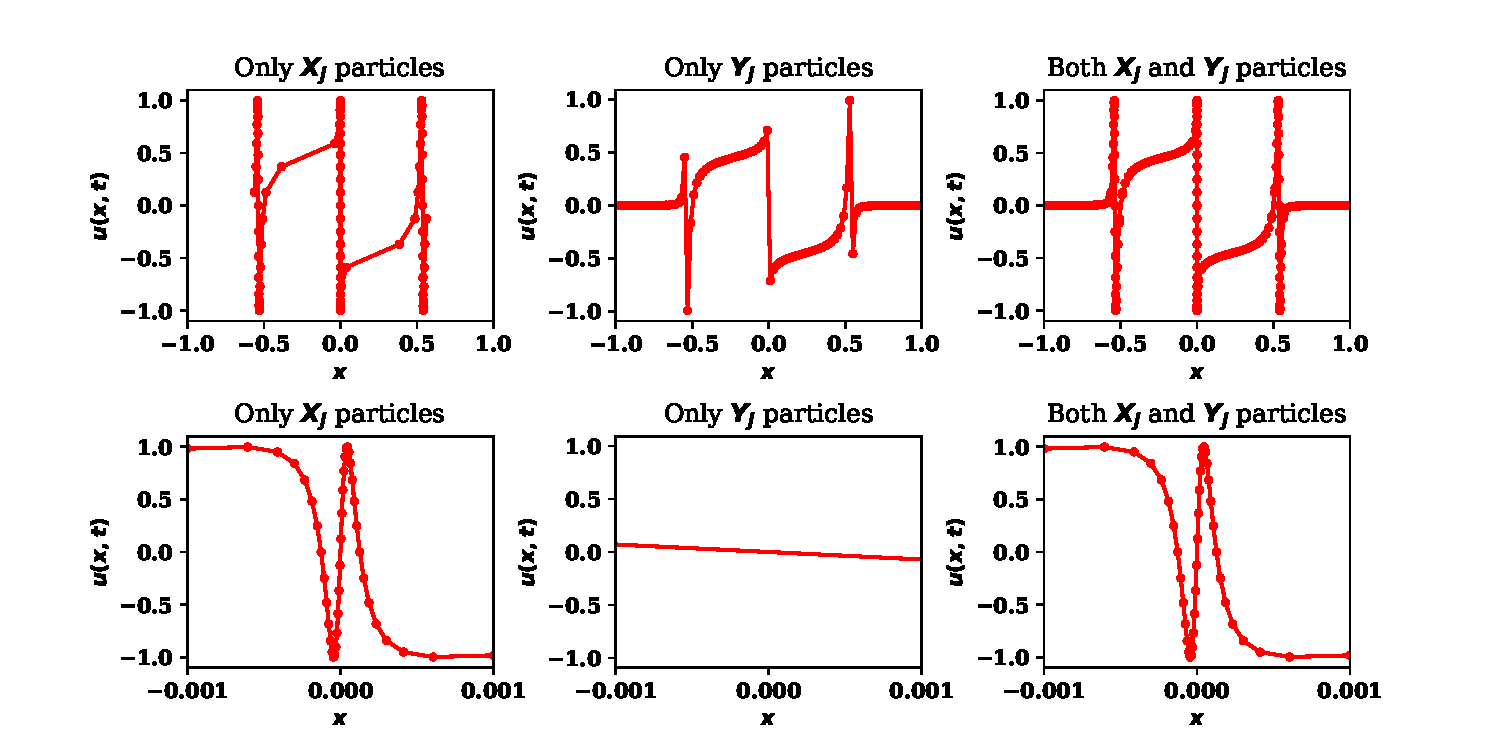
\includegraphics[width=\textwidth]{particle-plot.pdf}
  \caption{Demonstration that neither the particles $X_j(t)$ defined in \eqref{eq:Xj} nor the particles $Y_j(t)$ defined in \eqref{eq:Yj} are alone enough to fully describe the solution. Left figures: Solution plots obtained by only the $X_j$ particles. Center figures: Solution plots obtained by only the $Y_j$ particles. Right figures: Solution plots obtained by plotting both the $X_j$ and $Y_j$ particles. (I.e., formed by unioning the sets of particles.) Top plots: solutions obtained from pointwise values of $X_j$ and/or $Y_j$. Bottom plots: Inset with the solution viewed on the zoomed interval $[-10^{-3}, 10^{-3}]$. All experiments run to time $T = 1$ using the wavespeed and initial data in \eqref{eq:au0-1}, with $N = 100$ particles generated from an equidistant grid.}\label{fig:f1}
\end{figure}

  \section{Convergence}
  The method of characteristics paired with an ODE solver is a convergent numerical method under our assumptions. Let $T >0$ be given. Consider some fixed $x \in [-1,1)$. Define $X(T)$ as the solution to the ODE
    \begin{align}\label{eq:X-ode2}
      X'(t) &= -a(X(t)), & X(0) = x.
    \end{align}
    This ODE is the time-reversed version of \eqref{eq:Yj}, so that 
    \begin{align*}
      u(x,T) = u_0(X(T)).
    \end{align*}
    Now let $X_h(T)$ denote the computational approximation to $X(T)$ computed using an ODE solver with time step $h > 0$. Finally, define our approximate solution $u_h$ as
    \begin{align*}
      u_h(x,T) \coloneqq u_0(X_h(T)).
    \end{align*}
    Assume that our ODE solver is order-$p$ accurate, i.e., that
    \begin{align}\label{eq:ode-accuracy}
      \left| X(T) - X_h(T) \right| \leq C h^p,
    \end{align}
    where $C = C(a,T)$. Then the following result holds:
  \begin{proposition}\label{prop:convergence}
    With the above notation,
    \begin{align}\label{eq:pde-accuracy}
      \sup_{x \in [-1,1)} \left| u(x,T) - u_h(x,T) \right| \leq \widetilde{C} h^p,
    \end{align}
    where $\widetilde{C} = \widetilde{C}(a, T, u_0)$.
  \end{proposition}
  \begin{proof}
    Recall that we have assumed that $u_0$ is smooth, and hence it has a Lipschitz constant that is bounded by the $L^\infty$ norm of the derivative:
    \begin{align*}
      \left| u_0(x) - u_0(y) \right| &\leq U |x - y|, & U &= \sup_{x \in [-1,1)} |u_0'(x)|.
    \end{align*}
    Then,
    \begin{align*}
      \left| u(x,T) - u_h(x,T) \right| = \left| u_0(X(T)) - u_0(X_h(T)) \right| \leq U | X(T) - X_h(T)| \stackrel{\eqref{eq:ode-accuracy}}{\leq} C U h^p.
    \end{align*}
    Letting $\widetilde{C} = C U$ and taking the supremum over $x$ completes the proof.
  \end{proof}
  This result shows that the accuracy of the solution $u(x,t)$ computed via characteristics is governed entirely by (a) the accuracy of the ODE solver used to solve the characteristic equations, and (b) the Lipschitz constant of $u_0$. We numerically verify this result with the following example: consider \eqref{eq:wave} with 
  \begin{align*}
    a(x) &= -\sin(\pi x), & u_0(x) &= \sin(\pi x).
  \end{align*}
  We use a multi-stage Runge-Kutta integrator to numerically solve \eqref{eq:X-ode2}. In particular, we use a 5-stage low-storage integrator that is 4-th order accurate \cite{carpenter-kennedy-lserk}. Thus, we have the relation \eqref{eq:ode-accuracy} with $p = 4$. To verify that this accuracy is independent of $x$, we compute $L^\infty$ norms with respect to $x$ using the approximation,
  \begin{align*}
    \sup_{x \in [-1,1)} | u(x,T) - u_h(x,T) | \approx \max_{j=1, \ldots, 10^3} |u(x_j,T) - u_h(x_j,T)|,
  \end{align*}
  where $\{x_j\}_{j=1}^{10^3}$ is an equispaced grid on $[-1,1)$. To compute the exact solution $u(x_j,T)$, we use a method of characteristics solver with a very refined timestep.  Figure \ref{fig:f2} confirms that we achieve fourth-order accuracy with respect to the time step $h$ used in the ODE solver. 
\begin{figure}
  \begin{center}
  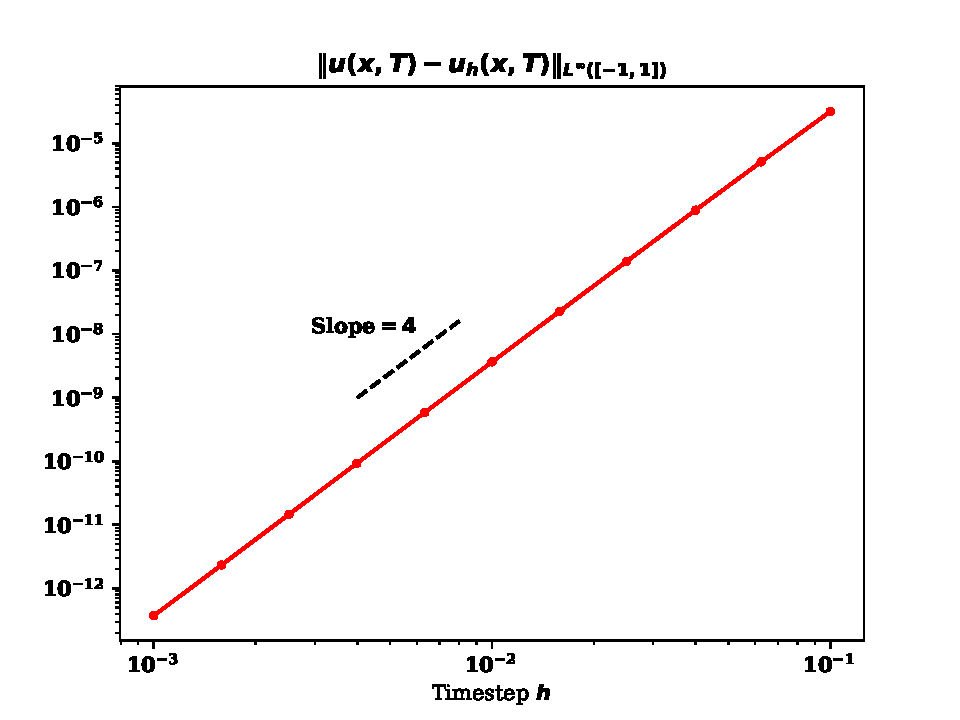
\includegraphics[width=0.6\textwidth]{convergence-plot.pdf}
  \end{center}
  \caption{Demonstration of Proposition \ref{prop:convergence}: the method of characteristics converges to the solution of a PDE pointwise with the same order as the characteristics ODE solver. We show pointwise error in the solution (computed as a maximum over a dense grid) using the method of characteristics with an ODE solver timestep $h$. Our solver is a fourth-order Runge-Kutta integrator, hence we expect fourth-order convergence, as shown in this plot.}\label{fig:f2}
\end{figure}

\bibliographystyle{siam}
\bibliography{references}

\end{document}
